\documentclass[12pt,letterpaper]{article}
\usepackage{graphicx,textcomp}
\usepackage{natbib}
\usepackage{setspace}
\usepackage{fullpage}
\usepackage{color}
\usepackage[reqno]{amsmath}
\usepackage{amsthm}
\usepackage{fancyvrb}
\usepackage{amssymb,enumerate}
\usepackage[all]{xy}
\usepackage{endnotes}
\usepackage{lscape}
\newtheorem{com}{Comment}
\usepackage{float}
\usepackage{hyperref}
\newtheorem{lem} {Lemma}
\newtheorem{prop}{Proposition}
\newtheorem{thm}{Theorem}
\newtheorem{defn}{Definition}
\newtheorem{cor}{Corollary}
\newtheorem{obs}{Observation}
\usepackage[compact]{titlesec}
\usepackage{dcolumn}
\usepackage{tikz}
\usetikzlibrary{arrows}
\usepackage{multirow}
\usepackage{xcolor}
\newcolumntype{.}{D{.}{.}{-1}}
\newcolumntype{d}[1]{D{.}{.}{#1}}
\definecolor{light-gray}{gray}{0.65}
\usepackage{url}
\usepackage{listings}
\usepackage{color}

\definecolor{codegreen}{rgb}{0,0.6,0}
\definecolor{codegray}{rgb}{0.5,0.5,0.5}
\definecolor{codepurple}{rgb}{0.58,0,0.82}
\definecolor{backcolour}{rgb}{0.95,0.95,0.92}

\lstdefinestyle{mystyle}{
	backgroundcolor=\color{backcolour},   
	commentstyle=\color{codegreen},
	keywordstyle=\color{magenta},
	numberstyle=\tiny\color{codegray},
	stringstyle=\color{codepurple},
	basicstyle=\footnotesize,
	breakatwhitespace=false,         
	breaklines=true,                 
	captionpos=b,                    
	keepspaces=true,                 
	numbers=left,                    
	numbersep=5pt,                  
	showspaces=false,                
	showstringspaces=false,
	showtabs=false,                  
	tabsize=2
}
\lstset{style=mystyle}
\newcommand{\Sref}[1]{Section~\ref{#1}}
\newtheorem{hyp}{Hypothesis}


\title{Problem Set 4}
\date{Due: November 26, 2026\\[0.5em]Emilia Lupi}
\author{Applied Stats/Quant Methods 1}


\begin{document}
	\maketitle
	\section*{Instructions}
	\begin{itemize}
		\item Please show your work! You may lose points by simply writing in the answer. If the problem requires you to execute commands in \texttt{R}, please include the code you used to get your answers. Please also include the \texttt{.R} file that contains your code. If you are not sure if work needs to be shown for a particular problem, please ask.
		\item Your homework should be submitted electronically on GitHub.
		\item This problem set is due before 23:59 on Thursday November 26, 2026. No late assignments will be accepted.
	\end{itemize}



	\vspace{.5cm}
\section*{Question 1: Economics}
\vspace{.25cm}
\noindent 	
In this question, use the \texttt{prestige} dataset in the \texttt{car} library. First, run the following commands:

\begin{verbatim}
install.packages(car)
library(car)
data(Prestige)
help(Prestige)
\end{verbatim} 


\noindent We would like to study whether individuals with higher levels of income have more prestigious jobs. Moreover, we would like to study whether professionals have more prestigious jobs than blue and white collar workers.

\newpage
\begin{enumerate}
	
	\item [(a)]
	Create a new variable \texttt{professional} by recoding the variable \texttt{type} so that professionals are coded as $1$, and blue and white collar workers are coded as $0$ (Hint: \texttt{ifelse}).
	
	\noindent First, I look at the variable \texttt{type} with \texttt{table()}, using \texttt{useNA = "ifany"} to also see the missing values. The variable has three categories: 44 blue collar occupations (\texttt{bc}), 31 professional occupations (\texttt{prof}) and 23 white collar occupations (\texttt{wc}). There are also 4 occupations with no type (NA). Then, I create the new variable \texttt{professional} with \texttt{ifelse()}. It takes the value 1 when \texttt{type} is equal to \texttt{"prof"}, and 0 when \texttt{type} is blue or white collar. Finally, I check the result with \texttt{table()} again. There are 31 professional occupations coded as 1 and 67 blue and white collar occupations coded as 0 ($44 + 23 = 67$), so the recoding is correct. The 4 occupations with no type stay as NA, because \texttt{ifelse()} cannot assign 1 or 0 to a missing value. These are removed before running the model in part (b).
	
	\lstinputlisting[language=R, firstline=48, lastline=50]{PS04_answersEL.R}
	
	\vspace{1cm}
	
	
	\item [(b)]
	Run a linear model with \texttt{prestige} as an outcome and \texttt{income}, \texttt{professional}, and the interaction of the two as predictors (Note: this is a continuous $\times$ dummy interaction.)
	
	\noindent First, I remove the missing values from the dataset with \texttt{complete.cases()}. This keeps only the rows with no NA in any column, so the 4 occupations with no type are removed and the model uses 98 occupations.
	
	\lstinputlisting[language=R, firstline=57, lastline=57]{PS04_answersEL.R}
	
	\noindent Then, I run the linear model with the \texttt{lm()} function. In the formula, \texttt{income * professional} is a short way of writing \texttt{income + professional + income:professional}. This means that R includes both variables on their own and also the interaction term between them, where \texttt{income:professional} is income multiplied by professional.
	
	\lstinputlisting[language=R, firstline=59, lastline=59]{PS04_answersEL.R}
	
	\noindent The results of the model are shown in Table \ref{tab:model_prestige}.
	
	
% Table created by stargazer v.5.2.3 by Marek Hlavac, Social Policy Institute. E-mail: marek.hlavac at gmail.com
% Date and time: Tue, Nov 24, 2026 - 22:46:01
\begin{table}[H] \centering 
  \caption{Regression of prestige on income and professional} 
  \label{tab:model_prestige} 
\begin{tabular}{@{\extracolsep{5pt}}lc} 
\\[-1.8ex]\hline 
\hline \\[-1.8ex] 
 & \multicolumn{1}{c}{\textit{Dependent variable:}} \\ 
\cline{2-2} 
\\[-1.8ex] & Prestige \\ 
\hline \\[-1.8ex] 
 Income & 0.003$^{***}$ \\ 
  & (0.0005) \\ 
  & \\ 
 Professional & 37.781$^{***}$ \\ 
  & (4.248) \\ 
  & \\ 
 Income x Professional & $-$0.002$^{***}$ \\ 
  & (0.001) \\ 
  & \\ 
 Constant & 21.142$^{***}$ \\ 
  & (2.804) \\ 
  & \\ 
\hline \\[-1.8ex] 
Observations & 98 \\ 
R$^{2}$ & 0.787 \\ 
Adjusted R$^{2}$ & 0.780 \\ 
Residual Std. Error & 8.012 (df = 94) \\ 
F Statistic & 115.878$^{***}$ (df = 3; 94) \\ 
\hline 
\hline \\[-1.8ex] 
\textit{Note:}  & \multicolumn{1}{r}{$^{*}$p$<$0.1; $^{**}$p$<$0.05; $^{***}$p$<$0.01} \\ 
\end{tabular} 
\end{table}  

	
	\vspace{1cm}
	\item [(c)]
	Write the prediction equation based on the result.
	
	\noindent Using the coefficients from Table \ref{tab:model_prestige}, the prediction equation is:
	\begin{equation*}
		\widehat{prestige} = 21.142 + 0.00317 \cdot income + 37.781 \cdot professional - 0.00233 \cdot (income \times professional)
	\end{equation*}
	
	\noindent Since \texttt{professional} can only be 0 or 1, the equation can be written separately for the two groups:
	\begin{align*}
		\text{Blue and white collar } (0): \quad \widehat{prestige} &= 21.142 + 0.003171 \cdot income \\
		\text{Professional } (1): \quad \widehat{prestige} &= (21.142 + 37.781) + (0.003171 - 0.002326) \cdot income \\
		&= 58.923 + 0.000845 \cdot income
	\end{align*}
	
	\noindent Because of the interaction term, the two groups have a different intercept and a different slope for income.
	
	\vspace{1cm}
	\item [(d)]
	Interpret the coefficient for \texttt{income}.
	
	\noindent The coefficient for \texttt{income} (0.00317) shows the effect of income for blue and white collar occupations only, i.e. when \texttt{professional} = 0. For these occupations, each additional dollar of average income is associated with a 0.00317-point increase in the prestige score, on average. This is about 3.17 points for every additional 1,000 dollars.
	
	
	\vspace{1cm}	
	\item [(e)]
	Interpret the coefficient for \texttt{professional}.
	
	\noindent When income is 0, professional occupations have a prestige score 37.781 points higher than blue and white collar occupations, on average. This value only holds for \texttt{income} = 0, because the interaction term makes the difference between the two groups change with income, as shown in part (g). However, no occupation in the data used for the model has an income of 0 (the lowest income is 1,656 dollars), so this coefficient has no real meaning by itself.
	
	\vspace{1cm}	
	\item [(f)]
	What is the effect of a \$1,000 increase in income on prestige score for professional occupations? In other words, we are interested in the marginal effect of income when the variable \texttt{professional} takes the value of $1$. Calculate the change in $\hat{y}$ associated with a \$1,000 increase in income based on your answer for (c).
	
		\noindent The marginal effect of income is the change in the predicted prestige score when income increases by one unit (one dollar), while \texttt{professional} is kept fixed. Because the model has an interaction term, this effect is not the same for the two groups, so we need to find it for professional occupations only. To do this, I set \texttt{professional} = 1 in the prediction equation from part (c):
	\begin{align*}
		\widehat{prestige} &= \hat{\beta}_0 + \hat{\beta}_1 \cdot income + \hat{\beta}_2 \cdot 1 + \hat{\beta}_3 \cdot (income \times 1) \\
		&= (\hat{\beta}_0 + \hat{\beta}_2) + (\hat{\beta}_1 + \hat{\beta}_3) \cdot income
	\end{align*}
	
	\noindent Grouping the terms in this way separates the intercept $(\hat{\beta}_0 + \hat{\beta}_2)$, which does not depend on income, from the slope $(\hat{\beta}_1 + \hat{\beta}_3)$, which is multiplied by income. Only the slope changes the predicted prestige when income changes, so the marginal effect of income for professional occupations is:
	\begin{equation*}
		\hat{\beta}_1 + \hat{\beta}_3 = 0.003171 + (-0.002326) = 0.000845
	\end{equation*}
	
	\lstinputlisting[language=R, firstline=89, lastline=89]{PS04_answersEL.R}
	
	\noindent This is the effect of a one dollar increase in income. To get the effect of a 1,000 dollar increase in income on the prestige score for professional occupations (\texttt{professional} = 1), I multiply the marginal effect by 1,000:
	\begin{equation*}
		0.000845 \times 1000 = 0.845
	\end{equation*}
	
	\lstinputlisting[language=R, firstline=93, lastline=93]{PS04_answersEL.R}
	
		\noindent To check this result, I plug values into the prediction equation, using as an example an increase in income from 6,000 to 7,000 dollars for a professional occupation:
	
	\lstinputlisting[language=R, firstline=96, lastline=100]{PS04_answersEL.R}
	
	\noindent The predicted prestige score is 63.995 when income is 6,000 dollars and 64.840 when income is 7,000 dollars, so the difference is $64.840 - 63.995 = 0.845$. This is the same as the marginal effect multiplied by 1,000. Since the line for professional occupations is straight, the result is the same for any 1,000 dollar increase, not only from 6,000 to 7,000. Therefore, for professional occupations, a 1,000 dollar increase in income is associated with a 0.845-point increase in the predicted prestige score, on average.
	
	\vspace{1cm}	
	\item [(g)]
	What is the effect of changing one's occupations from non-professional to professional when her income is \$6,000? We are interested in the marginal effect of professional jobs when the variable \texttt{income} takes the value of $6,000$. Calculate the change in $\hat{y}$ based on your answer for (c).
	
	\noindent In this case, the marginal effect of professional jobs is the change in the predicted prestige score when an occupation changes from non-professional (\texttt{professional} = 0) to professional (\texttt{professional} = 1), while income is kept fixed at 6,000 dollars. Because of the interaction term, the size of this effect depends on the level of income. To find it, I group the terms of the prediction equation from part (c) that are multiplied by \texttt{professional}:
	\begin{align*}
		\widehat{prestige} &= \hat{\beta}_0 + \hat{\beta}_1 \cdot income + \hat{\beta}_2 \cdot professional + \hat{\beta}_3 \cdot (income \times professional) \\
		&= (\hat{\beta}_0 + \hat{\beta}_1 \cdot income) + (\hat{\beta}_2 + \hat{\beta}_3 \cdot income) \cdot professional
	\end{align*}
	
	\noindent The first part $(\hat{\beta}_0 + \hat{\beta}_1 \cdot income)$ is the same for both groups, while the second part $(\hat{\beta}_2 + \hat{\beta}_3 \cdot income)$ is only added when \texttt{professional} = 1. So the marginal effect of professional jobs is $\hat{\beta}_2 + \hat{\beta}_3 \cdot income$. When income is 6,000 dollars:
	\begin{equation*}
		\hat{\beta}_2 + \hat{\beta}_3 \cdot 6000 = 37.781 + (-0.002326 \times 6000) = 37.781 - 13.954 = 23.827
	\end{equation*}
	
	\lstinputlisting[language=R, firstline=106, lastline=106]{PS04_answersEL.R}
	
	\noindent To check this result, I plug values into the prediction equation, computing the predicted prestige score for a non-professional and a professional occupation, both with an income of 6,000 dollars:
	
	\lstinputlisting[language=R, firstline=110, lastline=114]{PS04_answersEL.R}
	
	\noindent The predicted prestige score is 40.168 for a non-professional occupation and 63.995 for a professional occupation, so the difference is $63.995 - 40.168 = 23.827$. This is the same as the marginal effect computed above. Therefore, when income is 6,000 dollars, changing from a non-professional to a professional occupation is associated with a 23.827-point increase in the predicted prestige score, on average.
	
	\begin{figure}[H]
		\centering
		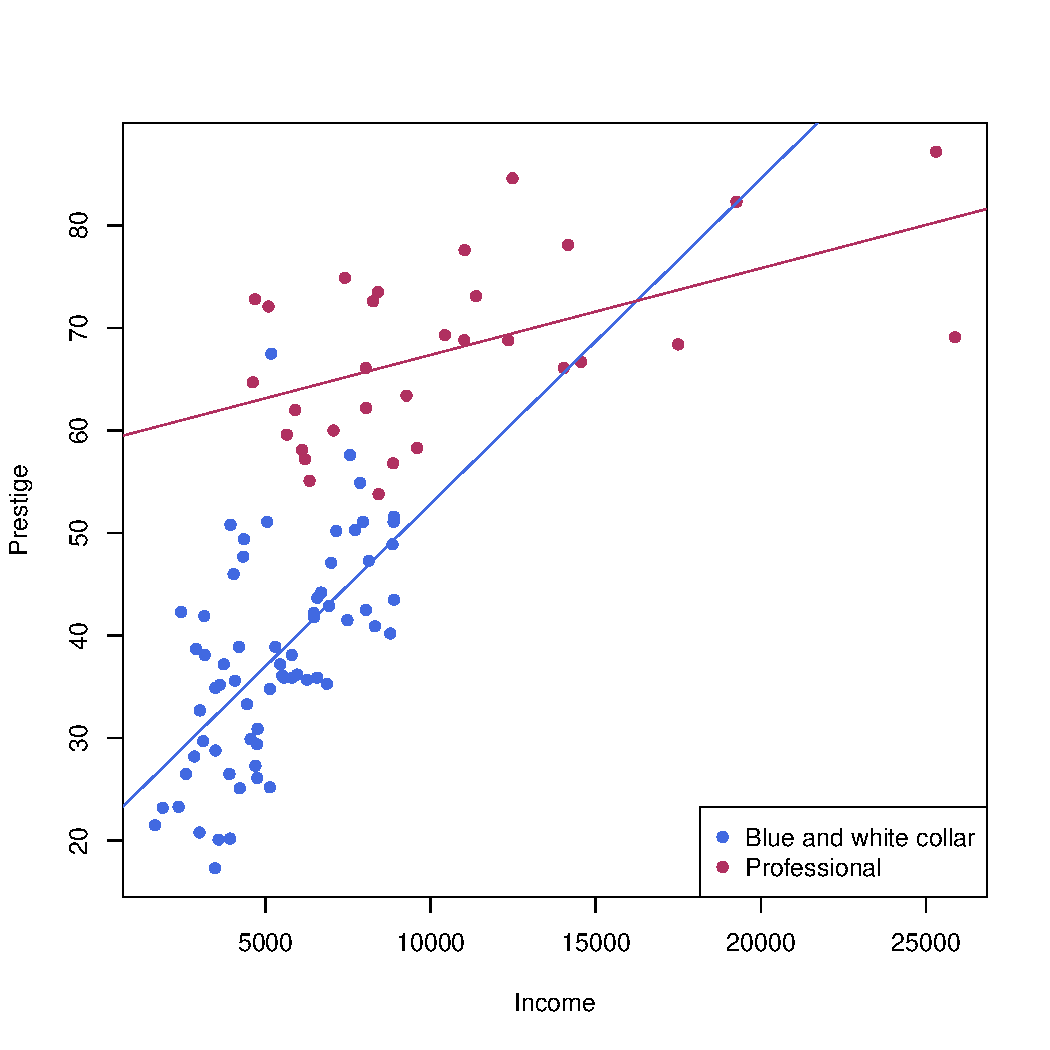
\includegraphics[width=0.75\textwidth]{plot_g.pdf}
		\caption{Predicted prestige by income for professional and non-professional occupations}
		\label{fig:plot_g}
	\end{figure}
	
	\noindent Figure \ref{fig:plot_g} shows the two regression lines from the model. The maroon line (professional occupations) starts higher but is flatter than the blue line (blue and white collar occupations), because the interaction term makes the effect of income smaller for professional jobs. This shows that the effect of being a professional is not fixed, but depends on income. 
	
	\noindent The marginal effect computed in this part is the vertical distance between the two lines at an income of 6,000 dollars. As income increases, the two lines get closer, so the advantage of professional occupations becomes smaller. The two lines cross at an income of about 16,245 dollars (where $37.781 - 0.002326 * income = 0$). Above this level the model predicts lower prestige for professional occupations. However, no blue and white collar occupation in the data has an income this high (the highest is about 8895 dollars), so this part of the line is an extrapolation and should not be read as a real result.
	
	
\end{enumerate}

	\vspace{1cm}	
\section*{Question 2: Political Science}
\vspace{.25cm}
\noindent 	Researchers are interested in learning the effect of all of those yard signs on voting preferences.\footnote{Donald P. Green, Jonathan	S. Krasno, Alexander Coppock, Benjamin D. Farrer,	Brandon Lenoir, Joshua N. Zingher. 2016. ``The effects of lawn signs on vote outcomes: Results from four randomized field experiments.'' Electoral Studies 41: 143-150. } Working with a campaign in Fairfax County, Virginia, 131 precincts were randomly divided into a treatment and control group. In 30 precincts, signs were posted around the precinct that read, ``For Sale: Terry McAuliffe. Don't Sellout Virgina on November 5.'' \\

Below is the result of a regression with two variables and a constant.  The dependent variable is the proportion of the vote that went to McAuliff's opponent Ken Cuccinelli. The first variable indicates whether a precinct was randomly assigned to have the sign against McAuliffe posted. The second variable indicates
a precinct that was adjacent to a precinct in the treatment group (since people in those precincts might be exposed to the signs).  \\

\vspace{.5cm}
\begin{table}[!htbp]
	\centering 
	\textbf{Impact of lawn signs on vote share}\\
	\begin{tabular}{@{\extracolsep{5pt}}lccc} 
		\\[-1.8ex] 
		\hline \\[-1.8ex]
		Precinct assigned lawn signs  (n=30)  & 0.042\\
		& (0.016) \\
		Precinct adjacent to lawn signs (n=76) & 0.042 \\
		&  (0.013) \\
		Constant  & 0.302\\
		& (0.011)
		\\
		\hline \\
	\end{tabular}\\
	\footnotesize{\textit{Notes:} $R^2$=0.094, N=131}
\end{table}

\vspace{.5cm}
\begin{enumerate}
	\item [(a)] Use the results from a linear regression to determine whether having these yard signs in a precinct affects vote share (e.g., conduct a hypothesis test with $\alpha = .05$).
	
	\noindent To test whether having lawn signs in a precinct affects vote share, I define the two hypotheses:
	\begin{align*}
		H_0&: \beta_1 = 0 \quad \text{(lawn signs have no effect on vote share)} \\
		H_a&: \beta_1 \neq 0 \quad \text{(lawn signs have an effect on vote share)}
	\end{align*}
	
	\noindent I perform a two-tailed t-test with $\alpha = 0.05$. First, I calculate the t statistic by dividing the coefficient by its standard error:
	\begin{equation*}
		t = \frac{\hat{\beta}_1 - 0}{SE(\hat{\beta}_1)} = \frac{0.042}{0.016} = 2.625
	\end{equation*}
	
	\noindent Then, I calculate the p-value from a t distribution with $n - k - 1 = 131 - 2 - 1 = 128$ degrees of freedom:
	
	\lstinputlisting[language=R, firstline=149, lastline=152]{PS04_answersEL.R}
	
	\noindent The p-value is 0.0097. Since $0.0097 < 0.05$, we reject the null hypothesis. This means that having lawn signs in a precinct has a statistically significant effect on vote share: precincts assigned lawn signs have a vote share for Cuccinelli about 4.2 percentage points higher, on average, than precincts not exposed to the signs.
	
	\vspace{1cm}	
	\item [(b)]  Use the results to determine whether being
	next to precincts with these yard signs affects vote
	share (e.g., conduct a hypothesis test with $\alpha = .05$).
	
	\noindent To test whether being next to precincts with lawn signs affects vote share, I define the two hypotheses:
	\begin{align*}
		H_0&: \beta_2 = 0 \quad \text{(being adjacent to lawn signs has no effect on vote share)} \\
		H_a&: \beta_2 \neq 0 \quad \text{(being adjacent to lawn signs has an effect on vote share)}
	\end{align*}
	
	\noindent I perform a two-tailed t-test with $\alpha = 0.05$. First, I calculate the t statistic by dividing the coefficient by its standard error:
	\begin{equation*}
		t = \frac{\hat{\beta}_2 - 0}{SE(\hat{\beta}_2)} = \frac{0.042}{0.013} = 3.231
	\end{equation*}
	
	\noindent Then, I calculate the p-value from a t distribution with $n - k - 1 = 131 - 2 - 1 = 128$ degrees of freedom:
	
	\lstinputlisting[language=R, firstline=157, lastline=160]{PS04_answersEL.R}
	
	\noindent The p-value is 0.0016. Since $0.0016 < 0.05$, we reject the null hypothesis. This means that being adjacent to precincts with lawn signs has a statistically significant effect on vote share: these precincts have a vote share for Cuccinelli about 4.2 percentage points higher, on average, than precincts not exposed to the signs.
	
	\vspace{1cm}
	\item [(c)] Interpret the coefficient for the constant term substantively.
	
	\noindent The constant term (0.302) is the predicted vote share for Cuccinelli when both variables in the model are equal to 0. This means precincts that were not assigned lawn signs and were not adjacent to precincts with lawn signs, so precincts that were not exposed to the signs at all. In these precincts, Cuccinelli got about 30.2\% of the vote, on average. Since the precincts were randomly assigned, this value works as the baseline (control group), and the coefficients in parts (a) and (b) show how much higher the vote share is in the precincts exposed to the signs compared to this baseline.
	
	\vspace{1cm}
	\item [(d)] Evaluate the model fit for this regression.  What does this	tell us about the importance of yard signs versus other factors that are not modeled?
	
	\noindent The model fit is measured with the $R^2$, which shows the share of the variation in the dependent variable that is explained by the model. The $R^2$ is 0.094, so the model explains only about 9.4\% of the variation in Cuccinelli's vote share across precincts. The other 90.6\% is explained by factors that are not in the model.
	
	\noindent This tells us that, even if the lawn sign variables are statistically significant (parts a and b), they explain only a small part of why the vote share is different between precincts.
	
\end{enumerate}  


\end{document}
